\chapter{人口空间流动网络分析}{Analysis of Population Spatial Floating Network}
人口流动是直接塑造城市间关系的重要动力,也是城市发展活力指标\cite{甄峰网络社会}。城市之间的
人口流动研究始终是人文地理学、城市地理学和经济地理学所关注的热点。现代社会发展,交通网络的日趋
发达将城市发展与人口流动紧密地联系在一起,人口活动不再局限于一个封闭的城市。从全球、国家或区域
层面来看,人口流动已经跨越了地理的限制。传统的人口流动的统计方法费时费力,社交网络应用使用LBS功能
为研究这列问题提供了新思路,通过新浪微博提供的API接口获取特定时间段内全国范围内发送微博的用户,根据用户
的账户位置信息和发送微博的位置信息,构建基于社交地理的人口流动网络,如图\ref{fig:floatinpopulation}所示。
\begin{figure}
  \centering
  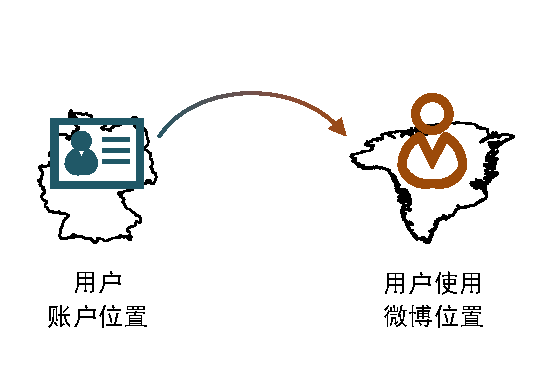
\includegraphics{figures/floating.pdf} \\
  \caption{流动示意图}{Floating illustration}
  \label{fig:floatinpopulation}
\end{figure}

\section{数据获取}{User Data Fetch}

新浪微博提供了place/nearby/users接口来获取附近发微博的用户,接口参数见表\ref{tab:poianduserapi}。
\begin{table}
  \centering
  \caption{NearbyUsers接口参数}{Nearby users api parameters}
  \label{tab:poianduserapi}
  \tabulinesep=1.5mm
  \begin{tabu}to 0.8\linewidth{X[1,c]X[1,c]X[2,c]}
    \tabucline[0.1em]-
    参数 & 类型 & 说明 \\
    \tabucline-
      lat & Float & 纬度 \\
      long & Float & 经度 \\
      starttime & Int64 & 开始时间 \\
      endtime & Int64 & 结束时间 \\
      range & Int & 查询半径,最大10km \\
    \tabucline[0.1em]-
   \end{tabu}
\end{table}

这些新浪微博用户数据包含了用户的名称、账号位置和用户当时所在空间位置,部分属性见格式见表\ref{tab:returnvalueuser}。
\begin{table}
  \centering
  \caption{用户地理空间位置(部分)}{Users' location information(partly)}
  \label{tab:returnvalueuser}
  \tabulinesep=1.5mm
  \begin{tabu}to 1.0\linewidth{X[1,c]X[2,c]|X[1,c]X[2,c]}
    \tabucline[0.1em]-
    属性 & 说明  & 属性 & 说明\\
    \tabucline-
    ID & 用户新浪微博ID & Name & 用户新浪微博名称 \\
    Province & 用户账户省份 & City & 用户账户城市 \\
    Lon & 用户位置经度 & Lat & 用户位置纬度\\
    \tabucline[0.1em]-
   \end{tabu}
\end{table}

春节前后是全国人口流动最为频繁的时间段,也是最能反映全国人口流动情况。因此选择$2016$年春节
前后$1$月$10$日和$2$月$10$日为起讫时间,获取全国微博用户位置数据,共$4.3$G,约$1500$万条用户记录。返回的数据为JSON格式,以键值的形式
保存表\ref{tab:returnvalueuser}中的属性,由于网络等其他问题,当请求量大的时候JSON数据中噪声较多,为了方便处理这些数据
因此将数据按行存放到HDFS中。

人口在不同城市之间流动构成了人口流动网络图,城市相当于网络图中节点,
不同城市之间人口流动相当于图中顶点之间的有向连接边,而人口流动数量则相当于边的权重。

GraphX作为Spark上层图处理模块,提供了并行化图分析算法。
为了方便分析城市人口流动分析,使用Spatial-Spark空间查询将全国数据抽象为一个Graph对象,
其中边$E_{ij}$为的权重为城市$j$中城市$i$用户的数量,算法流程图见\ref{fig:generateGraph}。
\begin{figure}
  \centering
  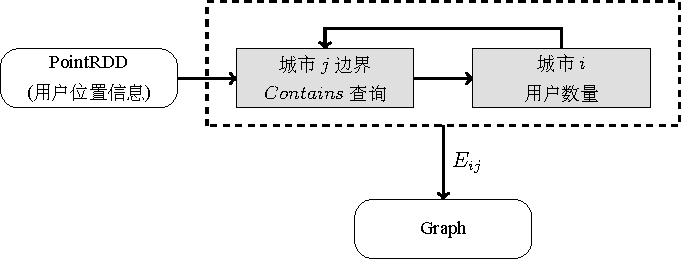
\includegraphics[scale=0.8]{figures/graph.pdf} \\
  \caption{Spatial-Spark生成人口流动网络图}{Generation floating population graph using Spatial-Spark}
  \label{fig:generateGraph}
\end{figure}

\section{人口流动统计}{Statistic of Floating Population}
\subsection{流动指数}

为了定量分析人口流动情况,定义如下指数:

\begin{description}
\item[流入量:]账户为其他城市在$i$城市发送微博的微博用户量,用$\delta_i$表示;
\item[流出量:]账户为$i$城市在其他城市发送微博的微博用户量,用$\omega_i$表示;
\item[流入流出比:]流入量/流出量,$\psi_i=\delta_i / \omega_i$。
\end{description}

\subsection{并行化设计}
GraphX丰富的图操作运算中\cite{Gonzalez2014GraphX},其中aggreateMessages是最核心最强大的接口,
该方法将边和其关联两个顶点作为一个Triplet进行整体并行处理,如图\ref{fig:triplet}所示,节点A和B以及它们之间的有向边
组成一个Triplet。首先进行类似map操作,将每个Triplet生成相应的消息,
发送关联的顶点,可以选择发送至目的节点,也可以选择发送至源节点;
然后对发送到同一个节点的消息进行reduce操作,进行合并操作。
\begin{figure}
  \centering
  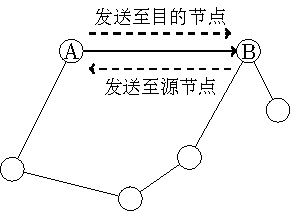
\includegraphics[width=0.4 \linewidth]{figures/triplet.pdf}\\
  \caption{Triplet操作示意图}{Triplet operations illustration}
  \label{fig:triplet}
\end{figure}

在计算城市人口流入量的时候,aggregateMessages接口中map操作选择将消息发送给有向边的目的节点;在计算城市
人口流出量的时候,map操作选择将消息发送给有向边的源节点,在reduce阶段所有消息汇总。
将上述两步生成的结果进行join和mapValue操作,计算每个城市的人口流动流出比,
算法流程见图\ref{fig:populationstatistic}。
\begin{figure}
  \centering
  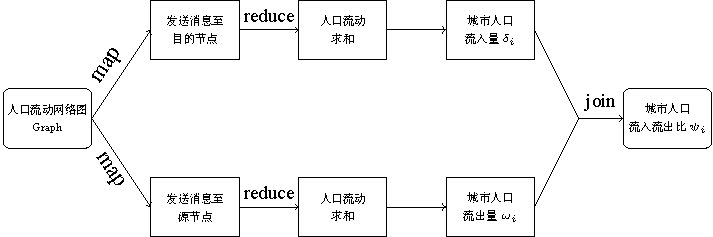
\includegraphics[width=0.9 \linewidth]{figures/population_statistic.pdf} \\
  \caption{人口流动统计流程图}{Flow chart of population statistic}
  \label{fig:populationstatistic}
\end{figure}

\subsection{统计分析}
以全国地级市和直辖市边界为空间查询范围,使用aggerateMessages函数分别计算出各自的流入量$\delta_i$、流出量$\omega_i$和流入
流出比$\psi_i$,结果栅格化渲染结果见图\ref{fig:flowinout}。
\begin{figure}
  \centering
  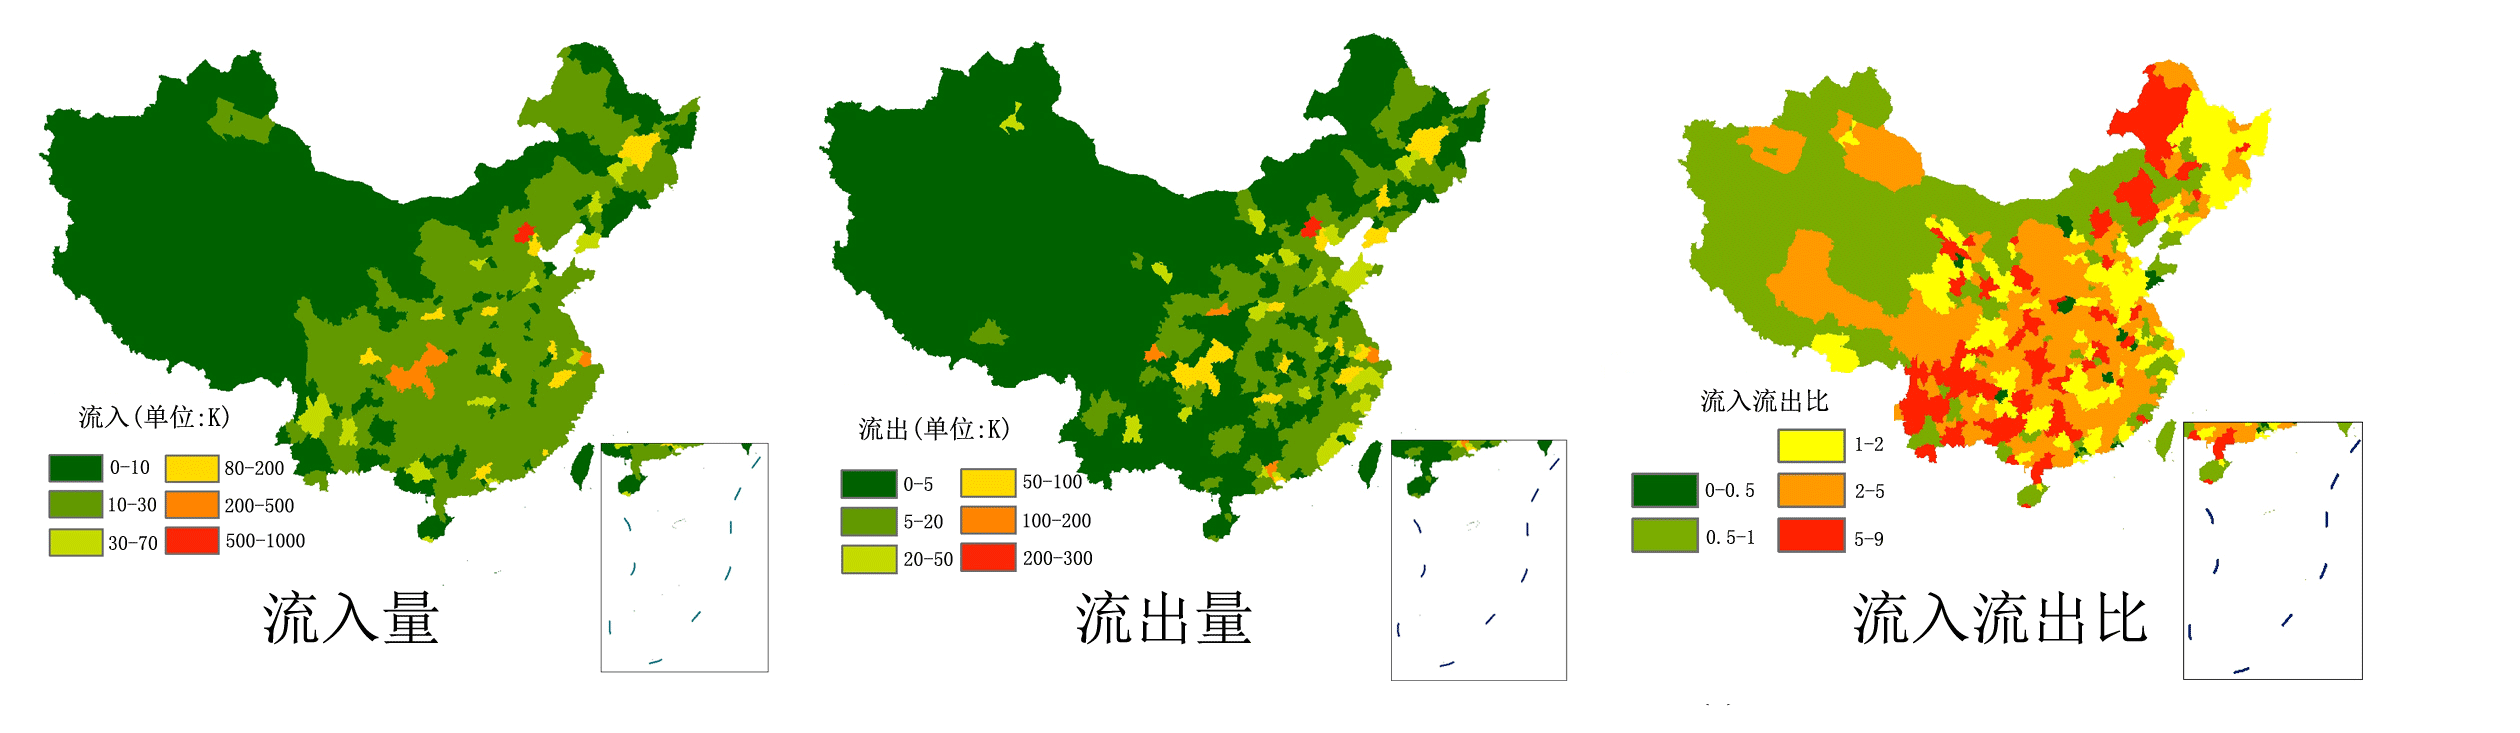
\includegraphics[width=13cm,height=4cm]{figures/flowratio.png} \\
  \caption{流出、流出和流入流出比}{Flow-in,flow-out and flow-ratio}
  \label{fig:flowinout}
\end{figure}

统计各个城市的人口流动数目,发现成都、西安、北京、广州、郑州等地为全国人口流动集中城市\cite{曹盼盼全国}。
并且人口流动量前$20\%$的城市占全国总用户的$70.1\%$,符合人口统计学和社会科学的「$80/20$法则」,
即$80\%$的事物或现象集中在前$20\%$的研究对象中。将前$20\%$城市人口流动统计见图\ref{fig:Populationstatistic},
可以看出人口流动流动量符合幂律分布(Power law)分布。
\begin{figure}
  \centering
  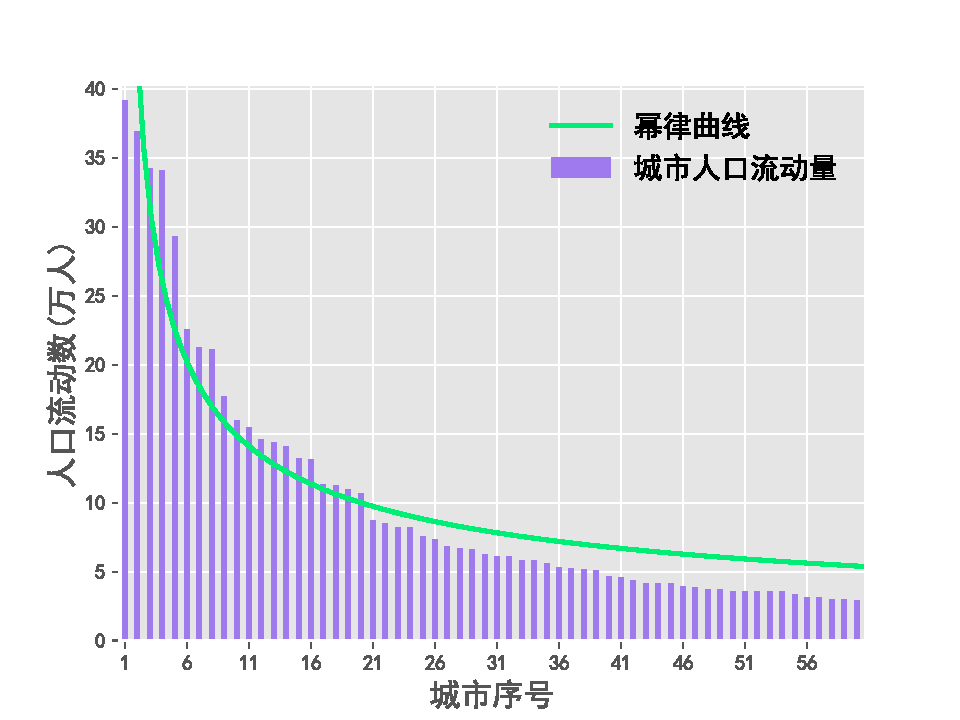
\includegraphics[scale=0.8]{figures/statisic.pdf} \\
  \caption{人口流动统计图}{Population flow statistic of cities}
  \label{fig:Populationstatistic}
\end{figure}

从图\ref{fig:flowinout}看出城市流入流出比呈现较多的复杂性:$\psi_i$远大于1表明该城市在春节期间人口呈现流入趋势;
$\psi_i$远小于$1$表明该城市在春节期间人口呈现流出趋势;而接近于$1$表明该城市人口在春节期间流动量持平,
主要城市的$\psi_i$见表\ref{tab:citiesinout}。
\begin{table}
  \centering
  \caption{城市流入流出比}{Cities' flow ratio}
  \label{tab:citiesinout}
  \tabulinesep=1.5mm
  \begin{tabu}to 1.0\linewidth{X[2,c,m]X[1,c,m]X[5,l,m]}
    \tabucline[0.1em]-
    \rowfont[c]{} 流入流出比$\psi_i$ & 说明 & 城市 \\
    \tabucline-
    大于1 & 流入 &   辽源、鄂州、西双版纳、毕节、永州、七台河、娄底、
                    姿阳、白色、黄冈、松原、三亚、娄底、大理等 \\
    接近1 & 持平 &  上海、北京、成都、武汉、哈尔滨、嘉兴、杭州、
                    长沙,广州、西安、太原、郑州、沈阳、乌鲁木齐等 \\
    小于1 & 流出 &  东莞、马鞍山、芜湖、青岛、苏州、深圳、包头、宁波、无锡、唐山,石家庄、呼和浩特等 \\
     \tabucline[0.1em]-
   \end{tabu}
\end{table}

流入流出比远大于$1$的城市主要有:\circled{1}春节返乡人群所在的城市,主要分布在人口劳动力输出的中西部城市,
四川、贵州、湖南、湖北等省份;剩余部分城市位于东北地区。\circled{2}南方著名旅游城市,海南,云南等省份。
随着旅游等第三产业发展,越来越多的人选择春节假期去度假,而不是回乡团聚,这些使得旅游城市在春节期
间迎来较大的人流量。

流入流出比接近$1$的城市春节期间人口流入量与流出量大致相同,这些城市主要是某个区域的连接中心,一般为省会城市,
如上海,北京,成都,武汉等等。

流入流出比小于$1$的城市主要有:\circled{1}沿海以劳动密集型产业发展起来的移民城市,集中在长三角和珠三角地区,据公安部最
新数据表明,深圳市常住人口超过$1300$万,但本地人口只有$250$万,外来人口超过$80\%$,位列全国第一,苏州以$50\%$外来人口排
名第二。\circled{2}重工业城市,其中以钢铁为代表重工业发展起来的城市如包头(包钢),唐山(首钢),马鞍山(马钢)等,人口
的流出可能与目前这些钢铁产业发达的城市产能过剩相关\cite{冯梅陈鹏钢铁}。

对人口流入流出比较大的城市,对这些城市交通、旅游等部门提供了决策依据,如航班的规划、旅游服务部门提前做好准备工作等等;也可以
通过从中人口的流入量,窥探城市经济走向和市场的活力。

\section{人口流向分析}{Analysis of Floating Population Route}

全国城市之间流动网络见图\ref{fig:citiesflow},从图中可以看出人口流向存在着不均衡性,明显的东部、中部和西部阶梯之分,
东部地区城市之间流动量大,流动密度强,中部地区次之而西部地区最小。
\begin{figure}
  \centering
  \includegraphics[scale=0.6]{figures/flow.jpg} \\
  \caption{城市人口流向}{Cities' population flow}
  \label{fig:citiesflow}
\end{figure}

\subsection{PageRank算法}
PageRank算法是Google搜索引擎的核心技术\cite{Boldi2009PageRank},该算法的核心思想
是将整个互联网抽象成网络图,每个网页抽象成一个节点,而节点之间的URL连接代表了网络图的边。
被许多重要页面引用的页面,往往还是重要的页面。算法开始假设所有节点拥有相同的权重,根据节点
的之间的链接权重设计出转移矩阵,通过权重转移矩阵相乘,重新分配权重,不停迭代循环,直至节点权重收敛。

以人口流动为例,将城市抽象成有向网络图中的各个节点,人口的流动抽象成节点之间的连通路径,构建出每个城市之间的流动矩阵$M$:

\[
  M=
\begin{bmatrix}
\alpha_{11} & \alpha_{12} & \ldots & \alpha_{1n} \\
\alpha_{21} & \alpha_{22} & \ldots & \alpha_{2n} \\
\ldots & \ldots & \ddots & \ldots \\
\alpha_{1n} & \alpha_{2n} & \ldots & \alpha_{nn} \\
\end{bmatrix}
\]

式中$\alpha_{ij}$为$i$城市人口流动至$j$城市的概率:
\begin{equation}
\label{eq:netprobability}
\alpha_{ij} = 
\left \{
  \begin{array}{cl}
  \frac{\beta_{ji}}{\sum_{k=0}^{k=n,k\ne i}\beta_{ki}} & i\ne j \\
  0 & i=j \\
  \end{array}
\right.
\end{equation}

式\eqref{eq:netprobability}中$\beta_{ki}$为在$k$城市微博用户中,账户位置为$i$城市的用户数量。
假设初始城市权重是相同的,即:
\begin{equation}
\label{eq:initalweight}
 V_0=
  \begin{bmatrix}
  1/n & 1/n & \ldots & 1/n 
  \end{bmatrix}^{T}
\end{equation}

通过$n$次迭代$V_n=M\times V_{n-1}$,直至$V_i$收敛,计算出每个城市在流动网络中的权重。

\subsection{城市流动网络权重}
GraphX模块中Graph类实现了PageRank算法,分为两种实现方式:一种是给定迭代次数的静态方法;另一种是给定
迭代收敛阈值的动态方法。本文选择动态方法,给定收敛阈值$0.0001$,计算得到权重前$20$位的城市见表\ref{tab:citiespagerank}。
\begin{table}
  \centering
  \caption{城市Pagerank排名}{Cities' Pagerank rank}
  \label{tab:citiespagerank}
  \tabulinesep=1.5mm
  \begin{tabu}to 1.0\linewidth{X[1,c]X[1,c]X[2,c]|X[1,c]X[1,c]X[2,c]}
    \tabucline[0.1em]-
    序号 & 城市 & PageRank值 & 序号 & 城市 & PageRank值 \\
    \tabucline-
    $1$ &   北京 & $0.058$ & $11$ & 厦门 & $0.014$  \\
    $2$ &   成都 & $0.033$ & $12$ & 哈尔滨 & $0.013$ \\
    $3$ &   上海 & $0.031$ & $13$ & 南京 & $0.012$ \\
    $4$	&   西安 & $0.028$ & $14$ & 长沙 & $0.012$ \\
    $5$ &   广州 & $0.026$ & $15$ & 沈阳 & $0.012$ \\
    $6$ & 	武汉 & $0.024$ & $16$ & 天津 & $0.011$ \\
    $7$ & 	杭州 & $0.017$ & $17$ & 长春 & $0.010$ \\
    $8$ & 	郑州 & $0.016$ & $18$ & 大连 & $0.009$ \\
    $9$ &	  深圳 & $0.015$ & $19$ & 济南 & $0.009$ \\
    $10$ &  重庆 & $0.014$ & $20$ & 太原 & $0.008$ \\
     \tabucline[0.1em]-
   \end{tabu}
\end{table}

以国家统计局2015年全国各直辖市、地级市和自治州的GDP数据,与城市人口流动网络权重进行相关性分析。
发现相关系数达$0.8$,表明呈现正相关关系,绘制散点图如图\ref{fig:rankgdpcorrelationanalysis}左
所示。为了更好的进行回归分析,将权重的平方根作为应变量,城市GDP数值作为响应变量,进行线性回归分析,结果如
图\ref{fig:rankgdpcorrelationanalysis}右所示,回归方程为:$\text{GDP} = 1.037\times 10^5 rank^{0.5}-2669$,
回归系数$\text{P-value} < 0.001$,通过假设检验。
\begin{figure}
  \centering
  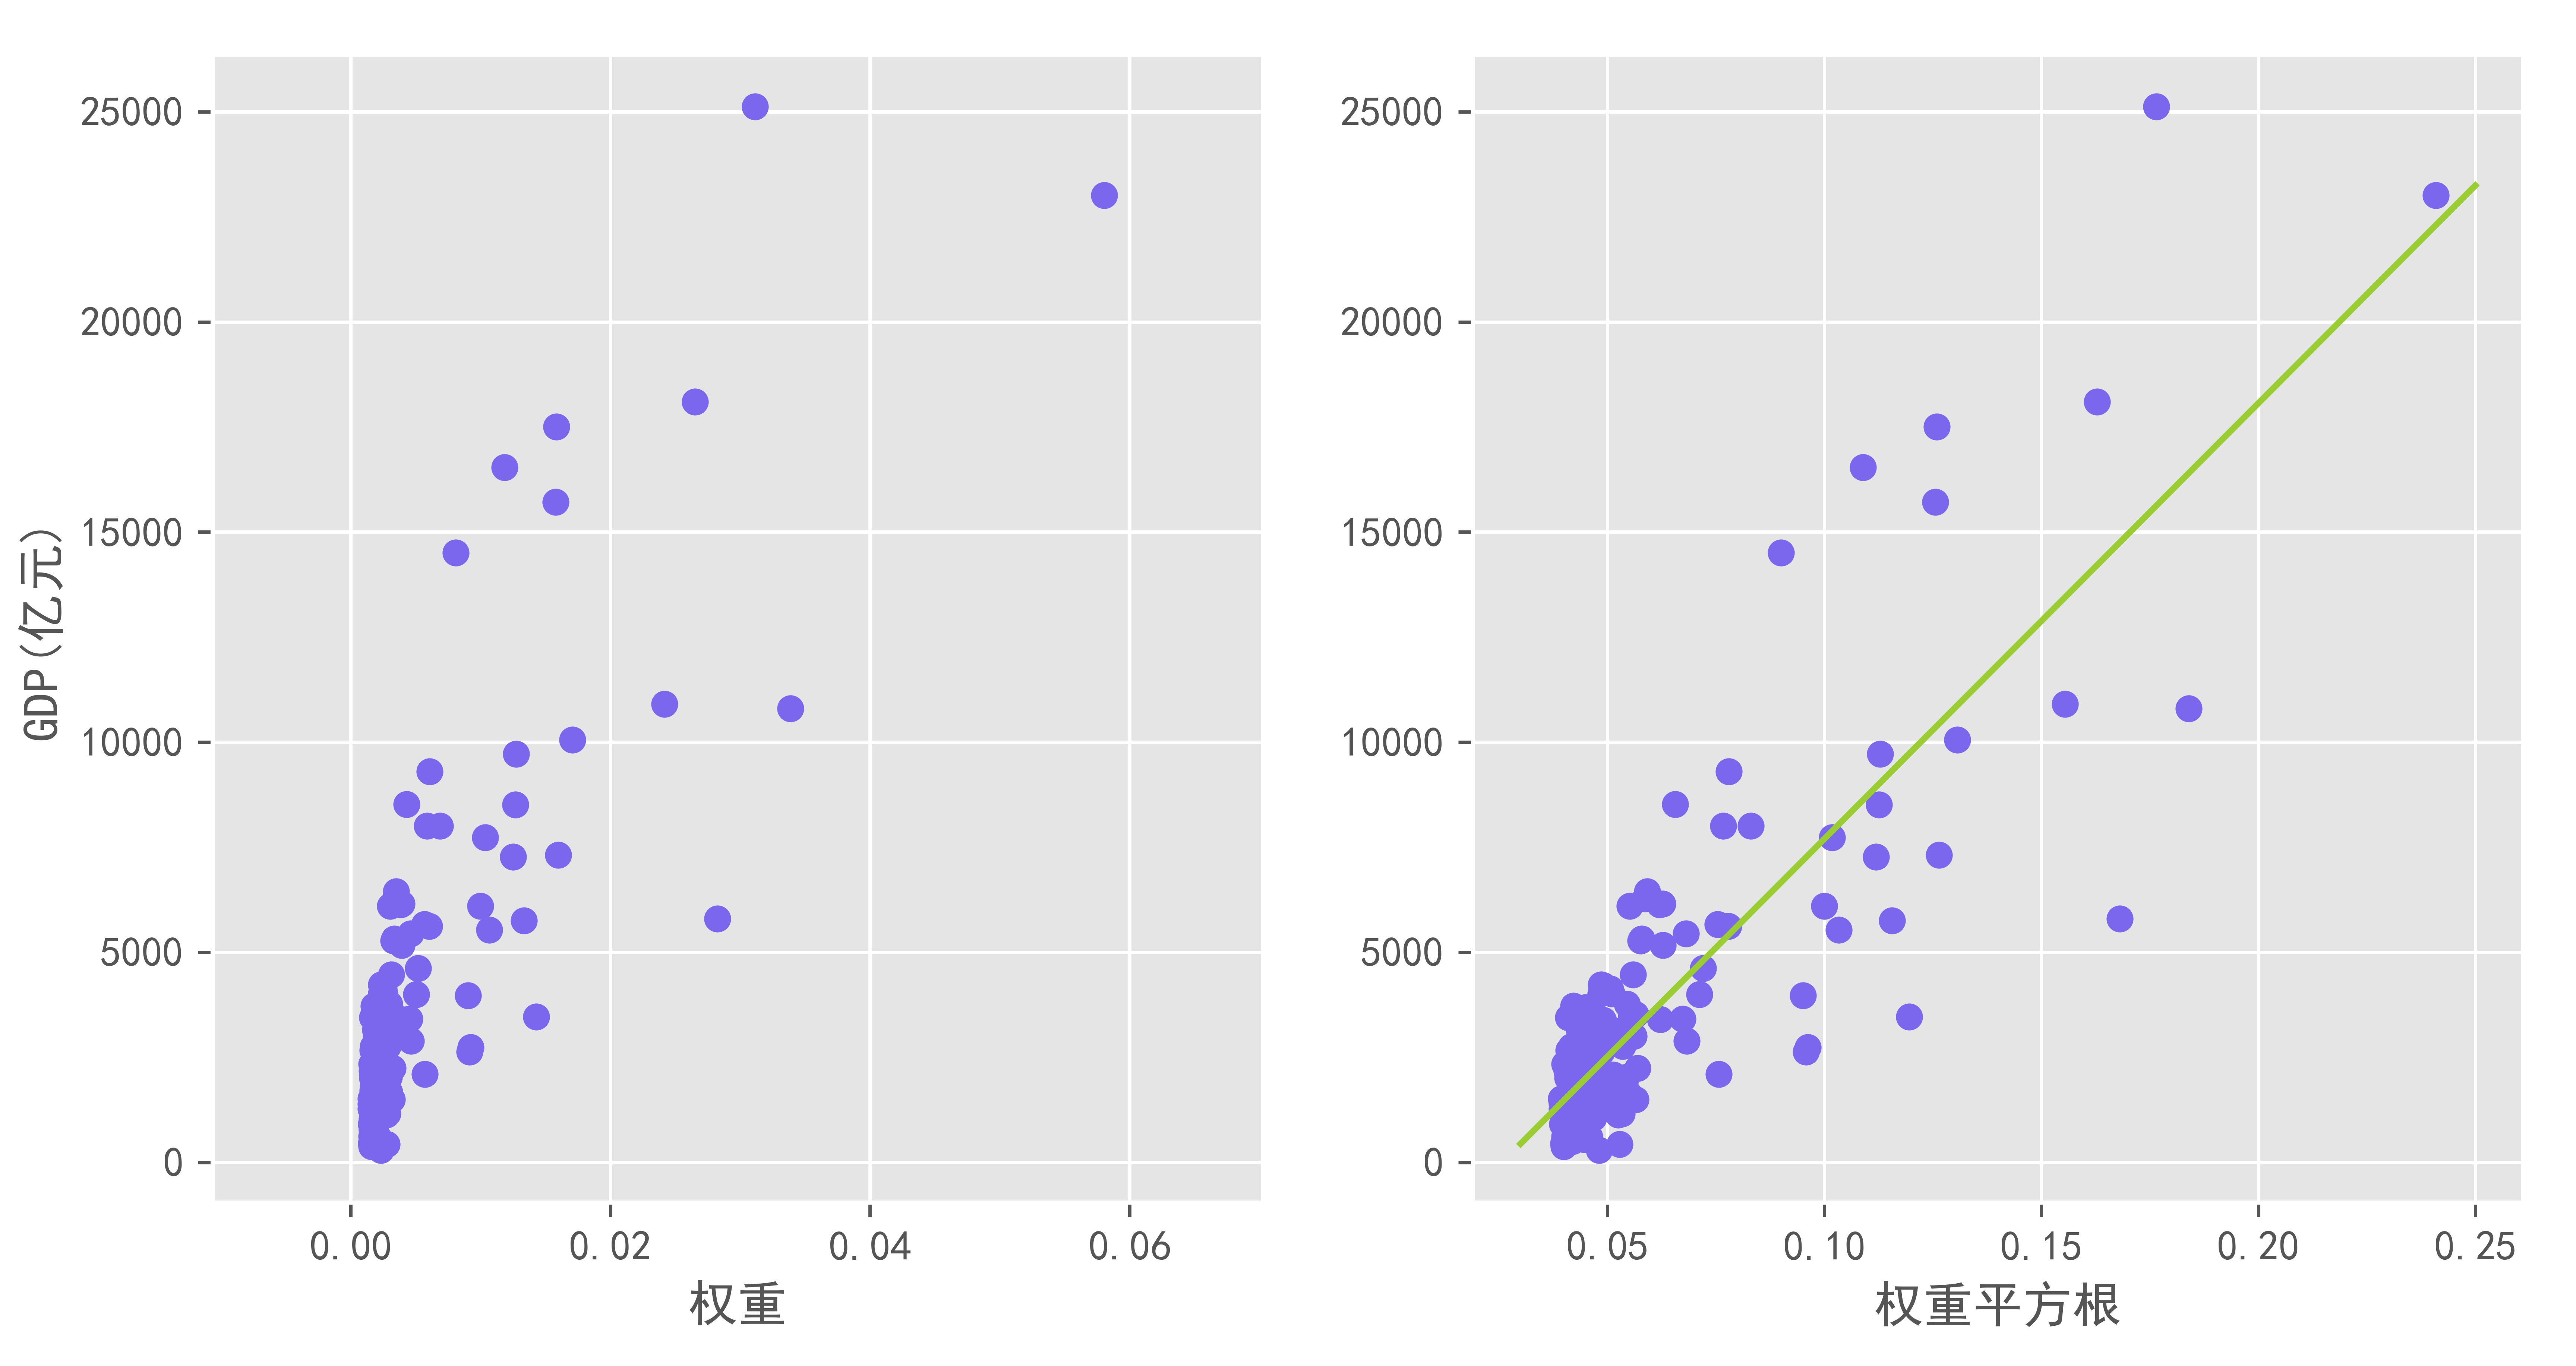
\includegraphics[scale=0.6]{figures/rank_gdp_scatter.png} \\
  \caption{权重和GDP相关性分析}{Ranks \& GDP correlation analysis}
  \label{fig:rankgdpcorrelationanalysis}
\end{figure}

从图\ref{fig:rankgdpcorrelationanalysis}中可以看出,并不是所有的点都很好的拟合回归曲线,存在「异常」
点。杠杆值可以描述点对整体回归的影响,高杠杆值可以说明改点属于异常点。据此绘制上述回归分析的残差平方与杠杆值散点图
,见图\ref{fig:residualLeverage},图中右下方和左上方的点属于异常点。
\begin{figure}
  \centering
  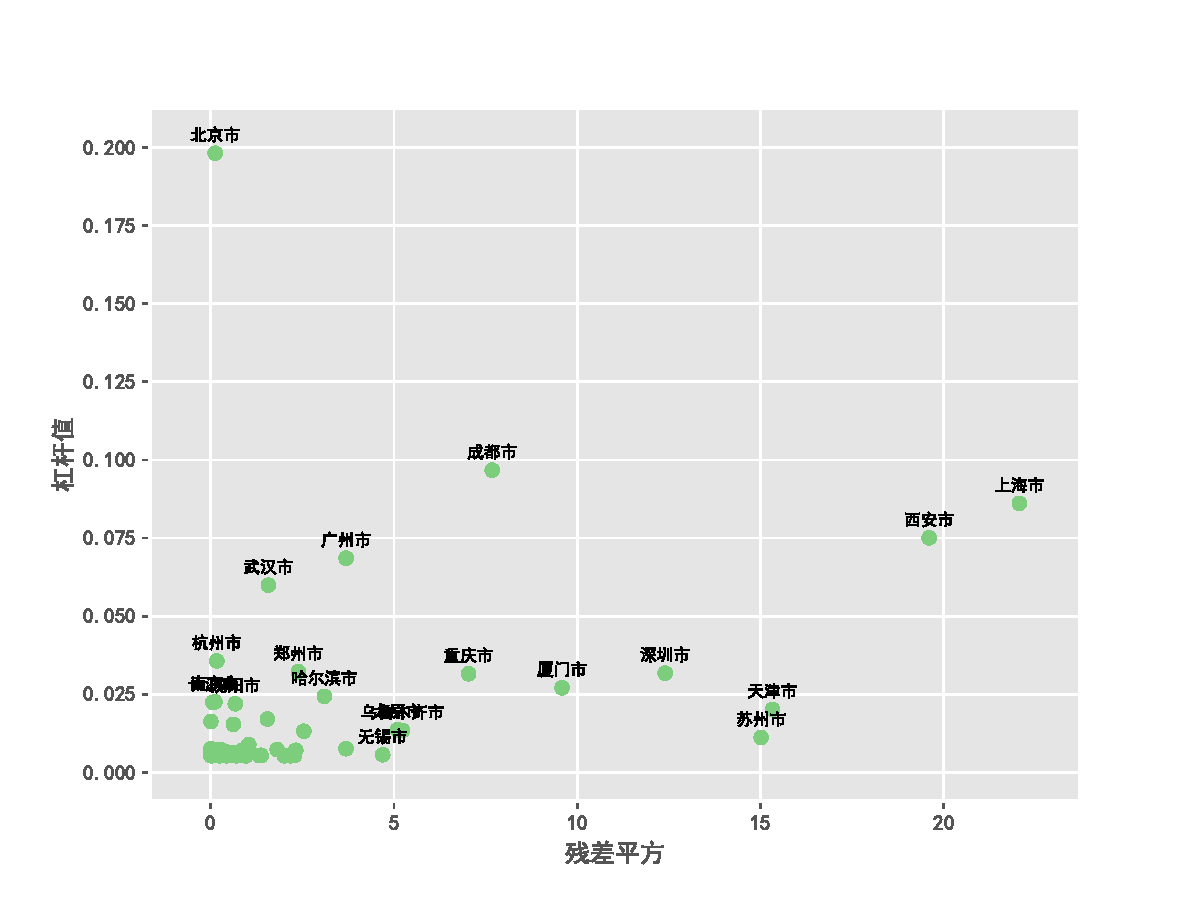
\includegraphics[scale=0.6]{figures/leverage.pdf} \\
  \caption{残差平方与杠杆值散点图}{Residual square \& leverage scatter plot}
  \label{fig:residualLeverage}
\end{figure}

城市特定时间段内在人口流动网络中的权重与实体城市权重存在明显的关系,出现了以下特征:

(1)城市权重与城市经济发展相对一致性。城市的权重与城市GDP呈现一定的正相关关系,
即城市的权重越高,城市的GDP数值会高。图\ref{fig:residualLeverage}中也表明了
在相关关系中异常点,主要分为两种:\circled{1}北京、成都、广州和武汉等城市权重
超出该城市GDP数值,其中北京最为明显;\circled{2}上海、西安、天津、苏州和深圳市等城市
的GDP发展远远大于该城市权重。

(2)城市权重在流动网络层级分布。通过对各个城市PageRank值分层,北京作为第一层级,是全国人口流动网络的中心;成都、上海、
西安、广州和武汉为第二个层级,是全国人口流动网络节点的副中心;杭州、郑州、深圳、重庆、厦门等为第三个层级,是区
域人口流动网络的中心;哈尔滨、南京、长沙、沈阳和天津等为第四个层级,是地区人口流动网络的中心。

(3)东部城市与中西部城市权重的差异明显。城市权重也符合「$80/20$法则」,排名前$20$城市权重和$0.81$。按照东部、中部、
西部三大地区划分,东部地区城市权重和$0.51$,中部地区城市权重和$0.32$,西部地区城市权重和$0.17$。虽然中部、西部地区也存在着权
重较高的城市,但东部区域在城市权重平均水平上明显高于中部和西部,因此东部城市在人口流动网络中扮演重要的角色。


\section{人口流动网络社群挖掘}{Community Mining of Floating Population Network}

现实世界中诸多系统都是以网络的形式存在,如人际关系网、机构协作网络、万维网等,这些统称为复杂网络(Complex Network),
可以通过简单的观测可以发现小规模网络的的特征、内部特征和划分,但是对于大规模和超大规模的网络,直观的显示很难通过肉眼发现
网络的特征和行为,因此需要使用复杂网络分析手段进行处理\cite{Girvan2002Community}。

网络社群挖掘(Community Mining,CM)是复杂网络聚类中研究最多的方法,社群挖掘方法对分析复杂网络中的拓扑结构,理解
复杂网络中隐藏的规律和预测复杂网络的行为不仅有重要的理论意义,而且有广泛的应用前景。城市之间人口流动也是属于一种复杂
网络,对该网络进行社群挖掘能够有效的发现城市在人口流动的联系,反映全国城市人口流动聚集效应。

\subsection{社群挖掘算法}

社群挖掘作为网络研究的经典问题,一直受到学者的广泛关注,目前社群挖掘算法主要有:GN(Girvan Newman)算法,定义边的介数,
依次删去介数最大的边,每次删除更新边的介数,如此循环,该算法在求解介数的时间复杂度较高\cite{Girvan2001Community};
LP(Label Propagation)算法使用邻居节点信息决定当前节点的社群,也可以应用到多社群挖掘,但是结果存在震荡问题,性能
不稳定\cite{Raghavan2007Near}。目前应用最多的是基于模块(Modularity)法,通过对比社群挖掘结果与随机图的差异判断社群划分的优劣,
研究表明基于模块值算法策略性能最好\cite{Newman2006Modularity}。

基于模块值算法通常先假设网络满足某种统计分布,进而通过极大似然估计方法得到网络社群。核心思想为模块值$Q$最大化,
见式\eqref{eq:qdefinition},$Q$是评价网络社群划分的优劣的质量指标。
\begin{equation}
\label{eq:qdefinition}
Q=\frac{1}{2m}\displaystyle{\sum_{vw}\big(W_{vw}-P_{vw}\delta(C_v,C_w)\big)}
\end{equation}

其中$W_{vw}$为网络中节点$v$和节点$w$之间的权重;$m$为权重之和;$P_{vw}$为零模型中节点之间的期望权重;$C_v$表示节点$v$所属的社群
的类别,如果节点$v$和节点$w$所属同一个社群,则$\delta(C_v,C_w)$为1,否则为0。

模块法开始将每个节点视为$N$个独立社群,选择使$Q$值增大最多或减少最小的连个顶点进行社群合并。
例如$A,B$连个社团合并,$a_i$为社团$A$中的成员,$b_j$为社团$B$中的成员,合并后的$Q$的
改变量用$\Delta Q$表示公式\eqref{eq:updateQ},$\Delta Q$为一个矩阵,其元素$e_{ij}$为社团$i$和
社团$j$合并后$Q$的变化值。%则社团合并后,因为合并无边相邻的社团对不能导致$Q$的增加,只需要考虑哪些相互之间有边的社团对。
\begin{equation}
\label{eq:updateQ}
\Delta Q_{AB}=Q_{AB}-Q_{A}-Q_{B}=\frac{1}{2m}\displaystyle{\sum_{a_i \in A, b_j \in B}}\bigg\{ \big( A_{ij} - \frac{k_ik_j}{2m} 
   \big) \times \delta \big[ r(i),r(j) \big] \bigg\}
\end{equation}

合并之后,对应的$\Delta Q$矩阵元素$e_{ij}$需要更新,如果选择让$A,B$社团合并为社团$D$,则新的社团$D$与其他社团之间(如社团$C$)
。在计算新一轮的合并$Q$时,易知$\Delta Q_{DC}=\Delta Q_{AC}+\Delta Q_{BC}$,上一次的迭代计算可以被
下一轮计算所采用,只需将$Q$矩阵中的$i,j$社团相关的行列相加,最多进行$n-1$次
计算来构建完整的社群划分\cite{Newman2012Communities}。

\subsection{社群挖掘算法并行化实现}

传统基于模块值社群挖掘算法是采用串行实现:逐个选择节点,选择合并社群,选择模块值最大的合并社群。而且需要两两考虑到
每个节点是否属于同一社群,算法时间复杂度将达到$O(n^2)$,当数据量急剧增加的时候,算法的时间消耗是可不接受的。因此
在并行计算框架下进行基于模块值进行社群挖掘,需要对公式\eqref{eq:qdefinition}简化为公式\eqref{eq:qdefinitionSimplify}。
其中$\sum_{in}$是社群$c$内部相互连接权重和,$\sum_{tot}$该社群$c$外部连接权重和。通过对比可以发现去掉了节点是否属于同一社群的判断
,避免了节点两两判断,简化了计算\cite{Blondel2008Fast}。
\begin{equation}
\label{eq:qdefinitionSimplify}
Q=\sum_{c}\big\{\frac{\sum_{in}}{2m} - (\frac{\sum_{tot}}{2m})^2\big\}
\end{equation}

判断某个节点$i$划分到其邻居节点计算模块值增益函数见公式\eqref{eq:updateQsimplify},其中$k_{i,in}$为节点$i$与社区$C$连接权重总和,
$k_i$为节点$i$与其余节点连接权重。
\begin{equation}
\label{eq:updateQsimplify}
\Delta Q=\big[ \frac{\sum_{in} + k_{i,in}}{2m} -(\frac{\sum_{tot}+k_i}{2m})^2 \big] 
      - \big[ \frac{\sum_{in}}{2m} - (\frac{\sum_{tot}}{2m})^2 - (\frac{k_i}{2m})^2 \big]
\end{equation}

算法主要分为两个步骤,第一步计算每个节点按照公式\eqref{eq:updateQsimplify}确定顶点$i$模块值增益最大进行合并社群,
第二步骤更新网络图,步骤见算法\ref{alg:communityMining}。
\begin{algorithm}[htbp]
\caption{社群挖掘算法}
\label{alg:communityMining}
\begin{algorithmic}[1]
\REQUIRE ~~\\
网络图:graph; \\
最多迭代次数: maxIterations;\\
模块值变化阈值: modularityThreshold;\\
\ENSURE ~~\\
模块值最大社群图: graph; \\
\STATE 初始化$C_i,\{i=1, 2,\ldots , N\}$
\STATE iterate=0
\WHILE{changeRate<modularityThreshold || iteration < maxIterations}
    \STATE changeRate=0
    \FORALL{$i$ in graph.vertexs} 
    \STATE $Q_i=[\quad ]$
    \FORALL{$j$ in $i$ neighbors}
    	\STATE $Q_i$ += $\Delta Q(i,j)$ $//$计算模块值增益
    \ENDFOR
    \STATE $Q_{max}$=max($Q_i$)
    \IF {$Q_{max} > 0$}
    	\STATE graph=updategraph() $//$如果最大模块值增益大于零,合并顶点
	\STATE changeRate= $Q_{max}$
    \ENDIF
    \ENDFOR
 \STATE iterate += 1 \\
\ENDWHILE
\RETURN graph
\end{algorithmic}
\end{algorithm}

算法\ref{alg:communityMining}每次迭代过程中依次选择图中的节点,对节点的所有的邻居节点尝试进行合并,对模块值增益最大且大于零的节点
进行合并。但是这种计算方式不利于并行计算框架,而且Spark RDD是不可变的数据结构,每次合并社群就要生成新的Graph对象,内存消耗非常大。
因此选择每次迭代更新多个节点,通过Graph类的aggregateMessages函数同时对图的所有边及其相关的节点进行同时操作,因此需要定义map阶段的
消息,按照公式\eqref{eq:updateQsimplify}的变量,定义如下消息结构。
\begin{lstlisting}[
  language=Java,
  morekeywords={implements, Integer, Long},
]
public class CombineMsg implements Serializable{
  public Integer degree;//该顶点的权重
  public Long commumity;//该顶点所属社区编号
  public Long commumityTotalDegree;//该社群权重总和
  public Long neighborDegree;//目标社群的权重
  public Long neighborCommumnity; //目标社群的编号
  public Long neighborCommumityTotalDegree;//目标节点的社群总权重
  public Long edgeWeight;//节点与与目标社群之间权重
}
\end{lstlisting}

对于发送到同一节点的消息集合,使用公式\eqref{eq:updateQsimplify},选择模块值增益值最大且大于$0$社群连边进行合并。
合并完毕后生成的消息图包含了本次社群合并连接顶点,并与原图进行joinVertice操作,完成图的更新。

由于所有边是并行操作,会出现「社群归属延迟」问题,如图\ref{fig:communityDelay}比如顶点$1$所在社群$c1$与顶点$2$所在社群$c2$进行合并,
而社群$c2$与顶点$3$所在社群$c3$进行合并,那么将会导致在joinVertice操作时候,这些顶点成为孤立的顶点。
从拓扑结构来看,社群$c1,c2,c3$应该属于同一个社群,因此对依据模块值增益生成的消息图计算连通分量,
直接使用Graph对象调用connectedComponents函数即可,最后与原图进行joinVertice操作,完成图的更新,流程示意图见图\ref{fig:Communitycombine}。
\begin{figure}
\centering
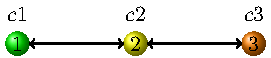
\includegraphics{figures/communitycombine.pdf}\\
  \caption{社群归属延迟}{Delay of commumity combine illustration}
  \label{fig:communityDelay}
\end{figure}

\begin{figure}
  \centering
  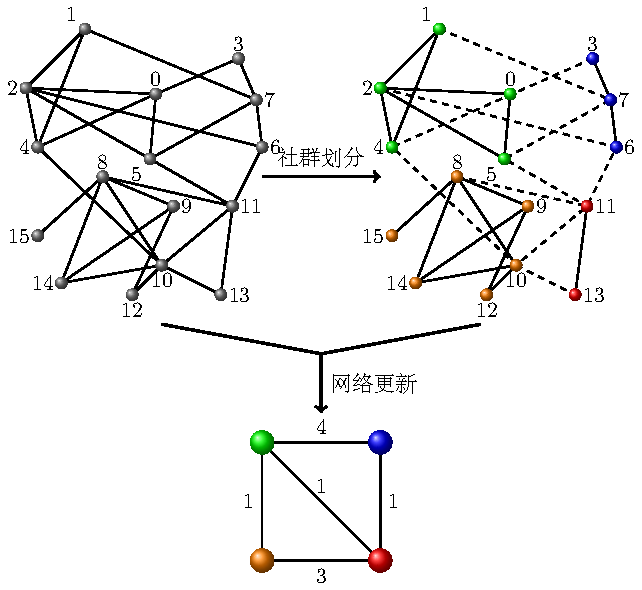
\includegraphics[scale=0.8]{figures/community.pdf}\\
  \caption{社群合并示意图}{Community combine illustration}
  \label{fig:Communitycombine}
\end{figure}

\subsection{城市社群挖掘}

由于人口流动往往存在较强的区域集聚性,在人口流动网络中体现出就是存在较强的社群结构,使用并行化
社群挖掘算法,反应全国城市人口流动的集聚效应\cite{杨小柳乡土中国}。对全国地级市和直辖市
人口流动网络进行社群挖掘,当整个人口流动网络划分为9个社群时,网络模块值最大,划分效果最好,
城市社群具体划分结果见图\ref{fig:nationalcommunitymining}和表\ref{tab:tbnationalcommunitymining}。
\begin{figure}
  \centering
  \includegraphics[width=10cm, height=8.115cm]{figures/commumity.jpg} \\
  \caption{全国城市社群划分}{National communities illustration}
  \label{fig:nationalcommunitymining}
\end{figure}
\begin{table}
  \centering
  \caption{全国城市社群划分详细}{National cities communities details}
  \label{tab:tbnationalcommunitymining}
  \tabulinesep=1.5mm
  \begin{tabu} to 1.0\linewidth{X[1,c,m]X[4,l,m]|X[1,c,m]X[4,l,m]}
    \tabucline[0.1em]-
    \rowfont[c]{} 社群&组成城市&社群&组成城市 \\
    \tabucline-
    1 & 北京、天津、河北城市、东三省城市、福建城市、三亚等 & 6 & 上海、江苏城市、安徽城市、浙江城市、丽江 \\
    2 & 山东城市 & 7 &广东城市、广西城市、湖南城市等\\
    3	& 河南城市	& 8	&重庆、四川城市、贵州城市等西南城市 \\
    4 & 山西城市 &	9 &	新疆城市、甘肃城市等西北城市 \\
    5	& 湖北城市、江西城市 & & \\
     \tabucline[0.1em]-
   \end{tabu}
\end{table}

对全国社群划分而言,也可以对其中的社群内部进一步使用社群挖掘算法,Spatial-Saprk强大的运算能力可以很容易的做到这一点,
比如上述全国社群1进一步使用社群挖掘算法,结果见图\ref{fig:subcommunity},每个社群中城市划见表\ref{tab:tabsubcommunity}。
\begin{figure}
  \centering
  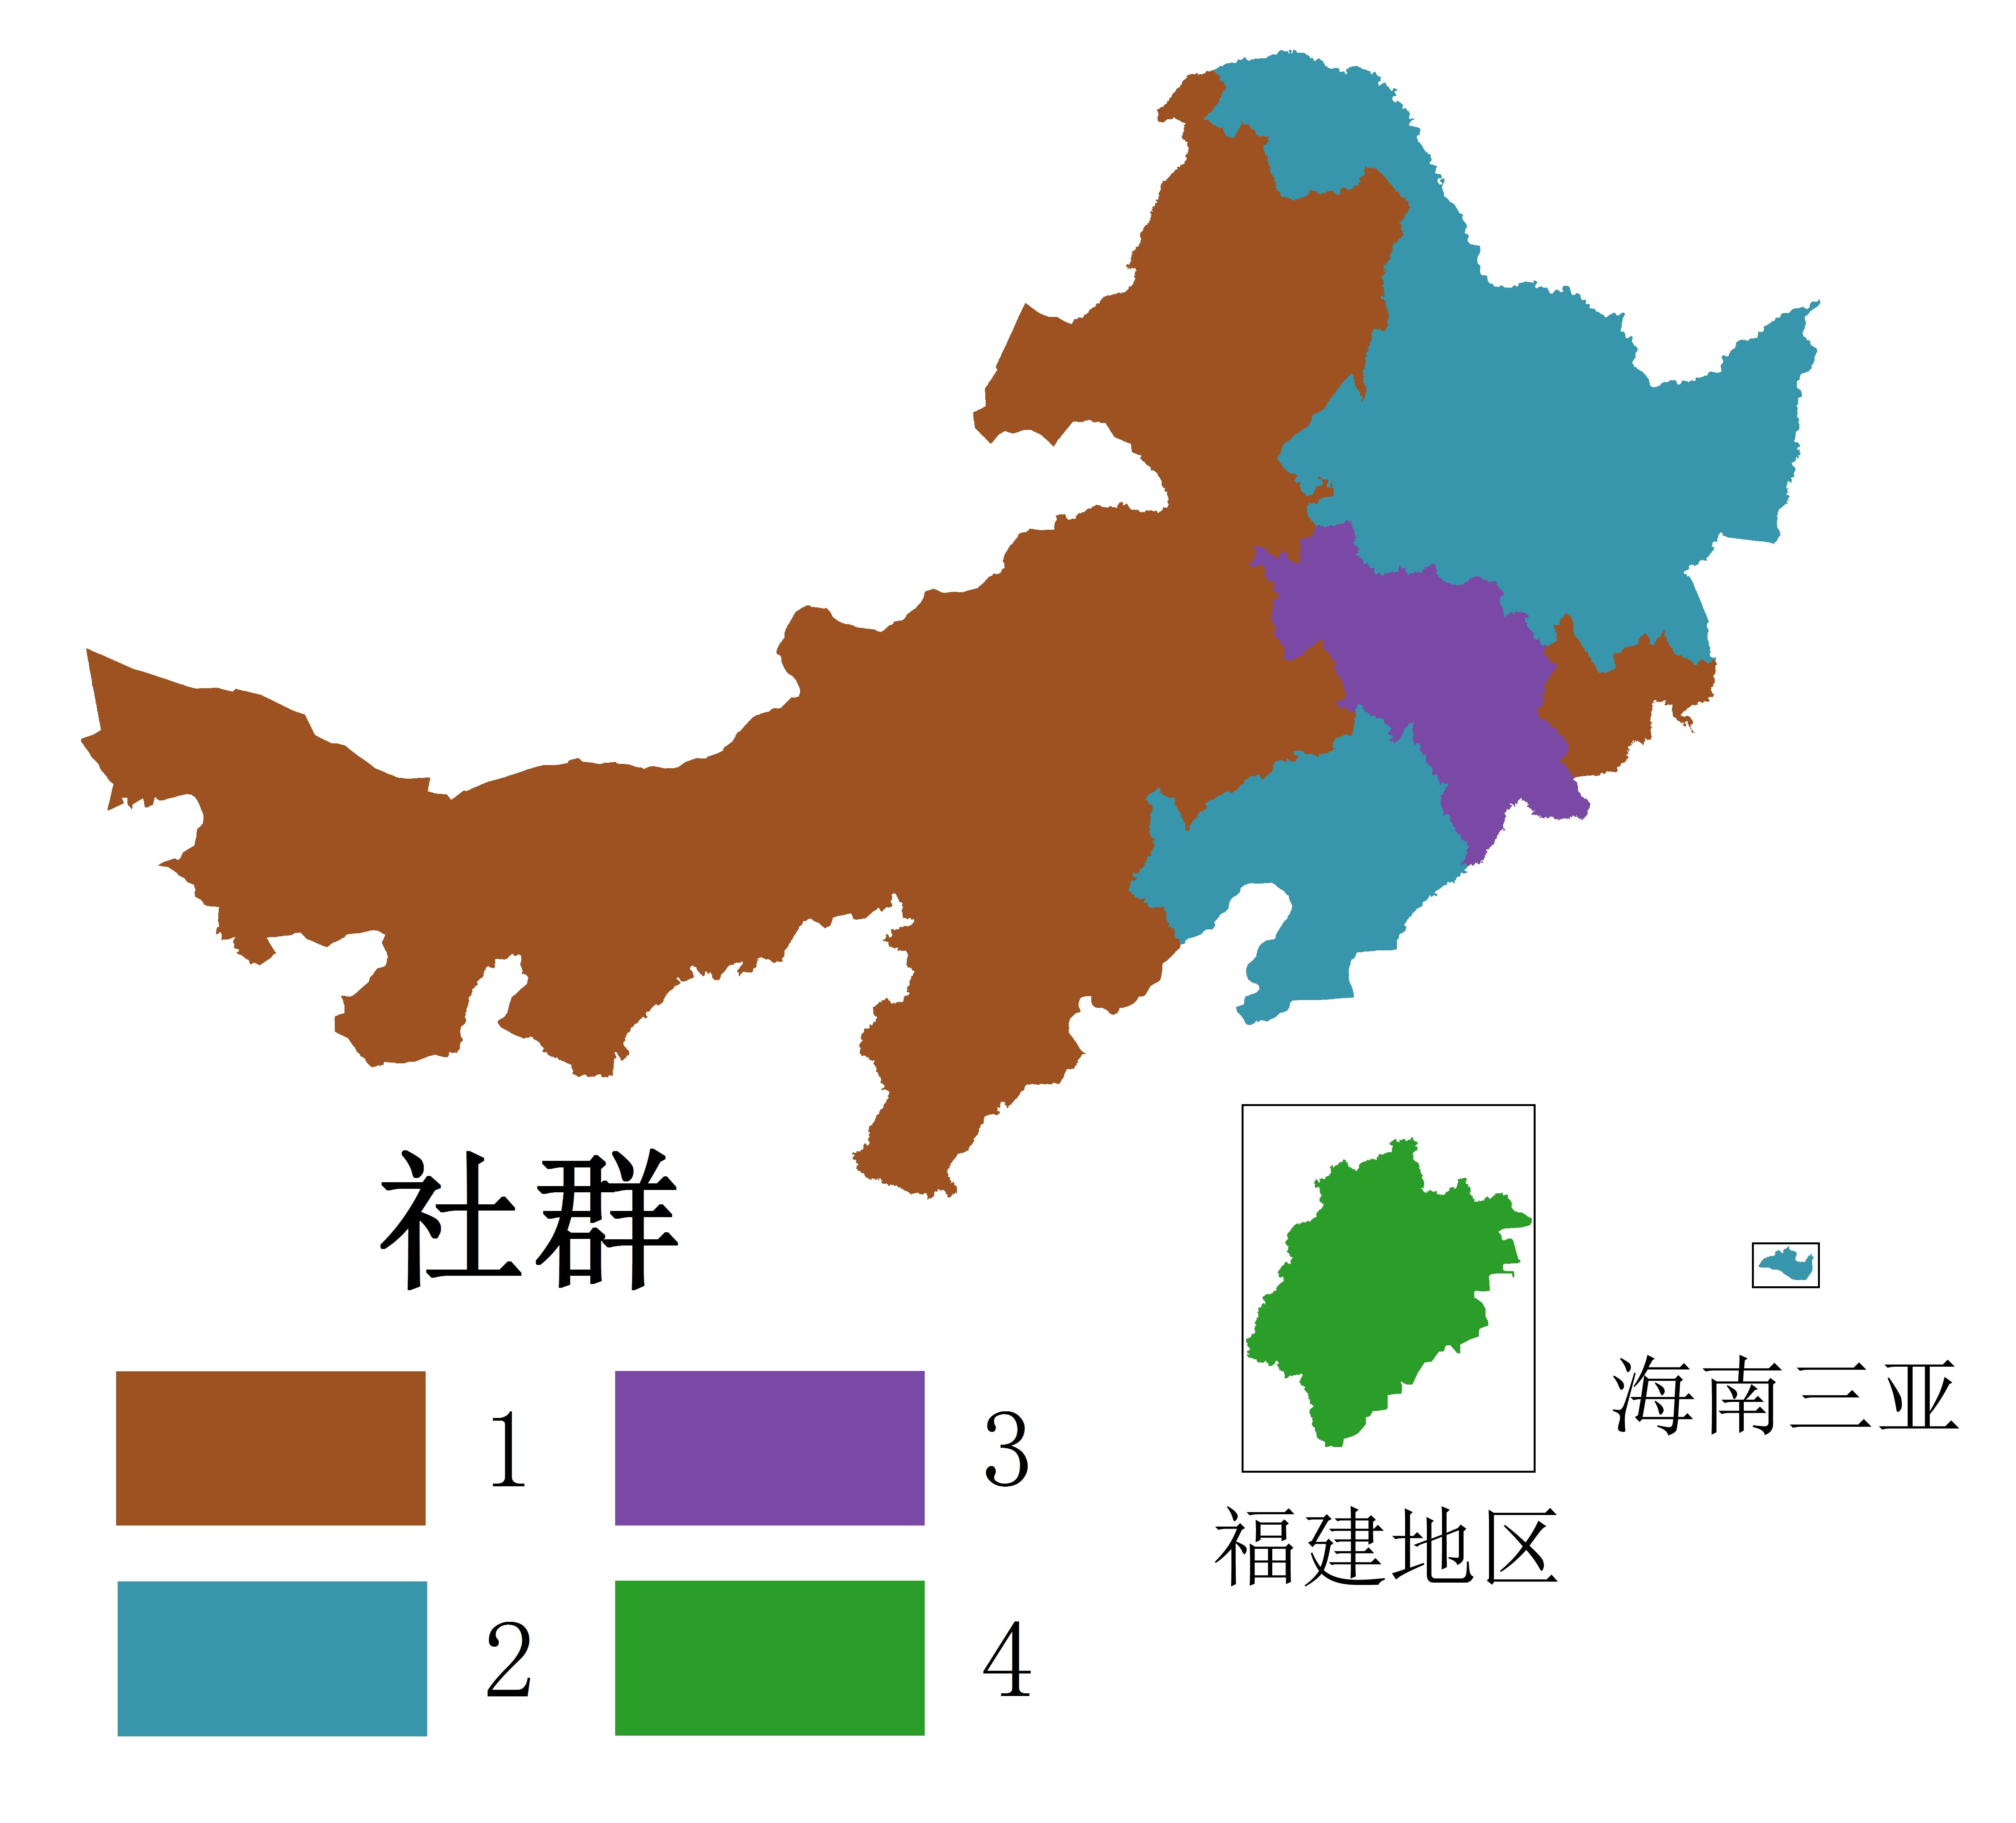
\includegraphics[width=8cm]{figures/subcommunity.jpg} \\ 
  \caption{子社群划分}{Sub-community illustration}
  \label{fig:subcommunity}
\end{figure}
\begin{table}
  \centering
  \caption{子社群划分}{Sub-community details}
  \label{tab:tabsubcommunity}
  \tabulinesep=1.5mm
  \begin{tabu} to 1.0\linewidth{X[1.2,c,m]X[6,l,m]|X[1.2,c,m]X[6,l,m]}
   \tabucline[0.1em]-
   \rowfont[c]{} 子社群 & 组成城市 & 子社群 & 组成城市 \\
    \tabucline-
   1 & 北京,天津,河北,内蒙古,吉林延边 & 2 & 黑龙江,辽宁,海南三亚 \\
   3 & 吉林城市 & 4 & 福建 \\
   \tabucline[0.1em]-
  \end{tabu}
\end{table}

分析每个社群的组成城市和城市之间地理空间分布,体现了以下特征:

(1)城市之间人口流动以省份为划分的特征较为明显,省份内部城市人口流动紧密
。以山东、山西、河南等省份为代表,其各自内部城市在人口流动网络中单独划分为一个社群。

(2)城市社群组成受地理空间位置影响较大,有明显的区域特征。在全国城市社群划分中,存在以北京为中心的
北方城市社群,上海为中心的东部城市社群,广东为中心的南部城市社群等集聚现象。

(3)城市社群组成也存在不受地理位置影响的特殊情况,如福建省的城市与北方城市组成同一社群,从侧面表
明其人口流动突破了地理空间的限制;丽江市与东部城市组成同一社群、三亚市与北方城市组成同一社群,
从一定程度表明这些旅游城市在春节假期的游客来源的组成。

(4)当对全国社群进行子社群进行社群挖掘,可以发现以省份为集聚现象越发明显,但是也可以发现少数城市与其他
省份人口联系更为密切,而这些往往是更值关注的内容,比如吉林的延边与北京、天津、河北等城市组成的社群更为
紧密,而海南三亚与黑龙江和辽宁组成的社群更为紧密。

通过对人口流动网络社群挖掘,可以快速地从海量数据中发现信息,这些信息既可以验证现实中已有的观念,如省份内部
人口流动紧密,空间邻近的省份人口交流频繁;也可以发现未知的现象,如福建省人口流动与北京、天津等省份城市
更为密切,海南三亚与北方城市尤其是黑龙江省份城市人口联系紧密。这些现象可以对省份和区域的决策者关于城市
规划、旅游航班调整、城市交通日常通勤等等方面提供很好的建议。

\section{本章小结}{Chapter Summary}

本章以全国新浪微博用户位置入手,构建了全国城市2016年全国城市人口流动网络,首先通过构建城市人口
流动指标,计算了城市人口流入、流出和流入流出比;借鉴PageRank计算每个城市在人口流动网络中的权重,
并与该城市GDP进行相关性分析,分析城市权重分布情况。最后对人口流动网络中进行社群挖掘,将全国城市
划分为9个社群,并分析了划分的特征。
